\section{The URDAD methodology}

The aim of URDAD is to provide a simple step-for-step, use-case driven analysis
and design algorithm which can be used by domain experts (e.g.\ business
analysts) to design processes (e.g.\ business processes) in a technology neutral
way. The resultant PIM is meant to be
mappable onto different implementation architectures and technologies.

%==================================================

\subsection{Methodology Requirements}

The outputs of the URDAD design methodology should comply to the PIM
requirements discussed in section \ref{sec:pimRequirements}. In addition the
methodology should be usable, simplifying the design
process and ensuring the consistency and quality of its outputs,
i.e.\ the methodology should satisfy the Berard requirements
\cite{berard:whatIsMethodology}.

In order to judge the quality of the outputs, one needs to specify the criteria
along which the quality of a design is judged.
Desired design qualities include simplicity
\cite{wirfs-brock:designSimplicity}, clean layers of granularity
\cite{martin:agileSoftwareDevelopment, artus:soaRealization},
flexibility and maintainability
\cite{hordijk:maintainabilityFactors,misra:drivingMaintainableDesign},
a high level of reusability \cite{lenz:softwareReuse}, and
testability across layers of granularity \cite{voas:softwareTestability}. In
addition, we require that the resultant design complies to the PIM
requirements specified in section  \ref{sec:pimRequirements}.

\begin{figure}
  \centering
  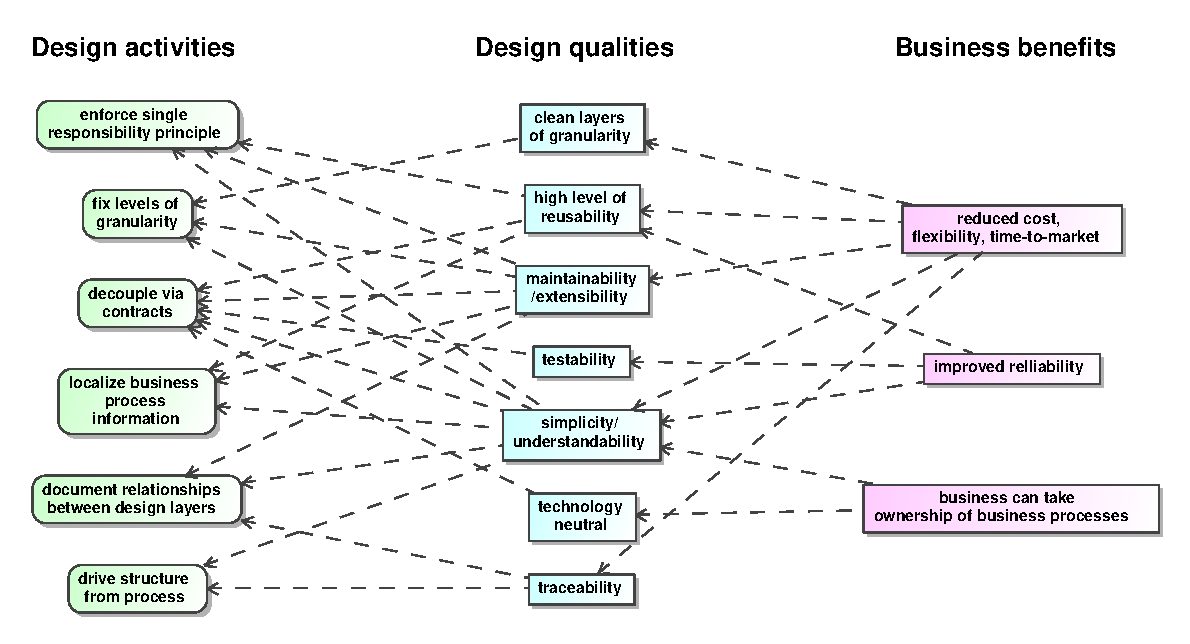
\epsfig{file=designActivities.eps, scale=0.6}
  \caption{Desired design qualities.}
  \label{fig:designActivities}
\end{figure}

Generating a design with the desired design qualities provides core business
benefits including improved flexibility and time-to-market,
improved reliability and the ability of business (instead of technology)
taking ownership of the business process designs.

%=================================================

\subsection{Design quality drivers}

We need to define an analysis and design algorithm which not only generates a
PIM which satisfies the PIM requirements, but one which also will exhibit
the desired design qualities.

Aiming to explicitly realize the design qualities is not necessarily an advisable
approach. For example,  one would often not want to
consciously design for, for example, re-usability. Such an approach would
necessitate that one would need to envisage potential future re-use scenarios.
This is not only a difficult task, but it also results in significant cost
overheads with uncertain returns and increased complexity. Instead one would want
to generate the simplest design solution which addresses the current requirements,
and achieve the qualities through a sound design process.

URDAD specifies a set of design activities which will drive out the desired
design qualities (see figure \ref{fig:designActivities}).
For example, the activities of enforcing the single
responsibility principle \cite{wirfs-brock:objectDesign,
wirfs-brock:responsibilityDrivenApproach}, decoupling via contracts
\cite{meyer:designByContract} and localizing the business process information
for any service at any level of granularity, one promotes reusability across
levels of granularity.

But, enforcing a contracts based approach not only drives re-usability, it also
improves simplicity and understandability (it is often sufficient to understand the
services contract without having to understand how the services contract is
realized) as well as testability (only once we have a solid services contract are we
really in a position to define service provider tests).

Figure \ref{fig:designActivities} shows the dependencies of the design qualities on
standard design activities enforced within the URDAD methodology. The details of
how these design activities generate a design with the desired design qualities
can be found in \cite{solms:urdad}.

Different role players may require, of course different design qualities. Business
management has indirectly an interest in all of these design qualities since they
all contribute to generating business value. They have a particular interest in
having technology neutral business process documentation across levels of granularity.
Project Management is particularly
concerned about traceability for estimation purposes and testability for status
reporting purposes. Business analysts require the simplicity and understandability
in order to be able to effectively work with business processes. Furthermore, clean
layers of granularity makes it easier for business analysts from different responsibility
domains to collaborate on a single business model. Implementors would like the freedom
to choose the implementation technologies, a high level of reuse and benefit from traceability,
testability and simplicity and understandability of the design.

%=================================================

\subsection{Analysis and technology-neutral design across levels of granularity}

URDAD is based on the view that both, analysis and design need to be done
across levels of granularity, i.e.\ that a single analysis phase generating
the functional requirements for a use case across levels of granularity
is not desirable. UML itself supports functional requirements across
levels of granularity via use case trees
with lower level functional requirements linked to higher level functional
requirements via {\em include} and {\em extend} relationships.
However, the analysis
and business process design across levels of granularity usually requires
business knowledge from different specialist domains and is hence often
performed across business analysts of various departments
contributing at different levels of granularity.

Furthermore, in the context of technology neutral design, the decision on
whether a particular domain of responsibility is to be hosted within the
organization or whether it is to be outsourced to external service providers is
only made when the implementation architecture is specified.

A technology neutral design methodology should thus support analysis and design
across levels of granularity, i.e.\ an analysis and a design phase for each
level of granularity.


%=================================================

\subsection{URDAD steps}

The steps of the URDAD methodology are shown in the first two swim lanes of
figure \ref{fig:methodology} while the implementation swim lane shows the
standard MDA steps for mapping the PIM onto an implementation.

\begin{figure}
  \centering
  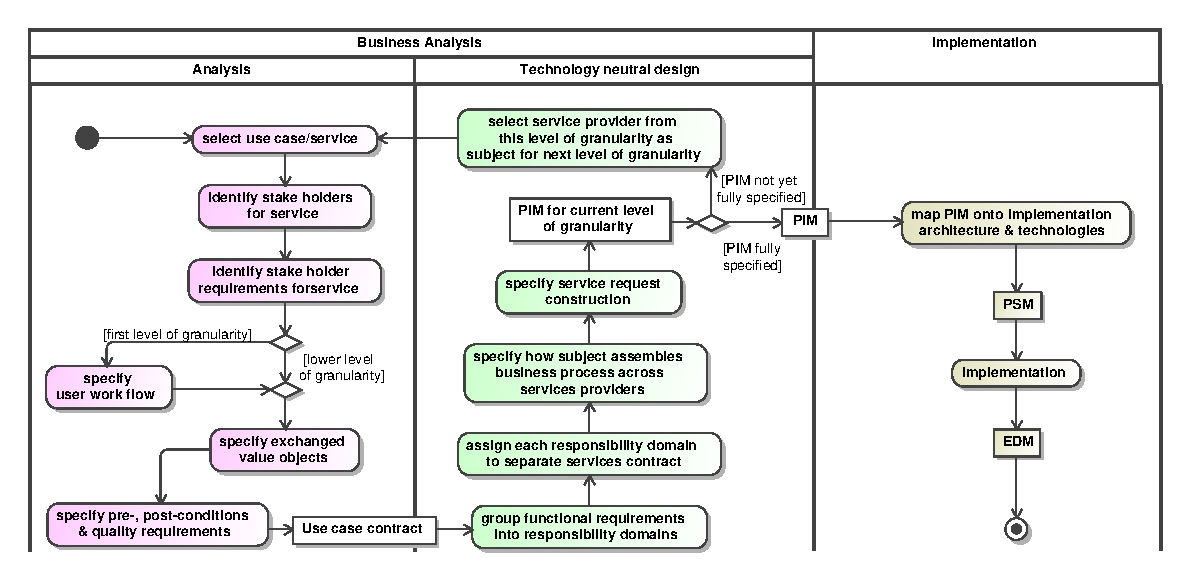
\epsfig{file=methodology.eps, scale=0.6}
  \caption{The URDAD methodology.}
  \label{fig:methodology}
\end{figure}

The process is iterative around use cases and incremental across levels of
granularity. Note that for each level of granularity there is both, an analysis
as well as a design phase. The output of the analysis phase is the use
case contract the functional and non-functional requirements for the use
case. The output of the design phase is the PIM for that level of
granularity containing the services contracts for the service providers
required for that level of granularity and the business process assembled
from these services.

%------------------------------------------------------

\subsubsection{The analysis phase of URDAD}

URDAD, like many other design and software development methodologies is use
case driven. The first step in the analysis phase is to identify
all the stake holders who have an interest in the use case and who will
potentially specify requirements for the use case.

During the second URDAD step one identifies the functional requirements for each stake
holder. It is in this early stage that the level of granularity is fixed by only including
direct functional requirements (i.e.\ not lower level functional requirements of functional
requirements). The lower level functional requirements will be addressed when capturing
the functional requirements for the lower level use cases/services.

In practice, one often tends to go too fine grained too quickly. This problem can be addressed
by explicitly checking whether
\begin{itemize}
  \item some functional requirements can be seen as lower level details of others,
  \item assessing whether some functional requirements can be grouped into a higher
			level functional requirement.
\end{itemize}

For the first level of granularity, one may need to define the user work flow
showing the sequences of messages exchanged between the user and the subject
for the various scenarios. When coming to lower levels of granularity, the
user work flow is already defined via the dynamics at the higher level of
granularity.

The next step is to specify the stake holder requirements around the value
(data) objects exchanged between the user and the service provider. As one
designs the business process across levels of granularity, one will identify
further information which is required and one will feed the appropriate
data structure elements into these data objects.

Finally one needs to formally specify the pre-conditions (the conditions under
which the service provider may refuse the service without breaking the
contract), the post-conditions (the conditions which need to be satisfied after
a successful completion of the use case) and the quality requirements (the
non-functional requirements like scalability, reliability, security, and
performance requirements).

The post-conditions are a formalization of the client's functional requirements,
i.e.\ each functional requirement placed by the client will be formally refined
by defining a testable post-condition.

The functional requirements, user work flow specification, data object requirements
together with the pre- and post-condition and quality requirements define the
use case contract.

%------------------------------------------------------

\subsubsection{The design phase of URDAD}

The first two steps of the design phase are those of grouping functional
requirements into responsibility domains and assigning them to services
contracts. For this we need to ask ourselves what domain is ultimately
accountable for a particular service, without concerning ourselves whether,
at lower levels of granularity the service will touch other domains of
responsibility. That will be addressed when we get to these levels of
granularity. It is thus not essential to ensure that
there is no overlap between domains of responsibility as
lower level functional requirements will be assigned to the appropriate responsibility
domains and ultimately to the service providers assigned to these domains of responsibility.


The responsibility identification and allocation steps enforce the single responsibility principle, the
contracts based approach and by locking into services contracts instead of
classes or objects, also the technology neutral aspect of the design.


The user itself may have to address certain responsibilities. If that is the
case, URDAD will also introduce a services contract for the user, specifying
formally the user responsibilities for the use case.

Having introduced services contracts for the responsibility domains to
be addressed for the use case, one now specifies how the business process is
assembled across the services provided by the services providers realizing these
services contracts.

Finally one projects out the collaboration context which shows the minimal structure
required to support the business process for the current level of granularity. Note
that the entity objects are also populated as information is required within a business
process. In this way URDAD aims to ensure that the design only has those structural
elements which are required for the execution of the business processes realizing the
stake holder requirements.

%------------------------------------------------------

\subsubsection{Transition to next lower level of granularity}

In order to go to the next lower level of granularity, one
selects one of the service providers from the current level of granularity
as new subject. The services become the use cases for the analysis phase
of this level of granularity. One now repeats the process by first identifying
the stake holders who have an interest in this lower level service or use case,
and subsequently their functional requirements.
One thus repeats the steps of the analysis and design phase for this lower
level of granularity, omitting the user work flow specification as this is
provided by the previous (next higher) level of granularity.

%------------------------------------------------------

\subsubsection{Lowest level of granularity}

The lowest level of granularity is reached if either a particular domain
of responsibility is outsourced, or if the functional requirements need not be
refined any further. In either of these two cases one ends with a services
contract specifying pre- and post-conditions (using the OCL) and quality
requirements for the services.

Low level services which perform simple transformations or calculations are
fully specified via post-conditions specified in OCL, i.e.\ the post-conditions
have sufficient information in order for their implementation to be autogenerated.

\subsection{Navigating the PIM}

UML tools enable one to conveniently navigate across the views within a particular level of granularity and to traverse across levels of granularity. This is further simplified
by stereotyping the various model elements using the URDAD UML Profile.

%---------------------------------------------------------

%\subsection{The URDAD meta-model}  ################################

%The URDAD meta-model defines a set of standard artifacts. The semantics for these artifacts
%is introduced in a UML profileintroducing the following concepts:
%\begin{itemize}
%  \item {\em :} Stake-holder, User, Service-provider, Observer, Entity, Services-contract,
%			Workflow-controller.
%  \item {\em Relationships:} Service for use case, Activity-for-service.
%  \item {\em Diagrams:} Functional requirements, user work flow specification,
%			services contract specification, responsibility allocation, business.
%			process specification (either sequence or activity diagram).
%\end{itemize}